\chapter{Examining MongoDB Query Features}
%Intro\footnotemark\\
\par In this Chapter, we will use the data stored in the "moviedetails.bson" file relating to
information on several films.

\begin{spacing}{0.9}
%note en bas de page
\section{Restoring a .bson file }
\par We start by restoring the “cinema” data in the MongoDB.
\begin{figure}[!htb] 
\begin{center} 
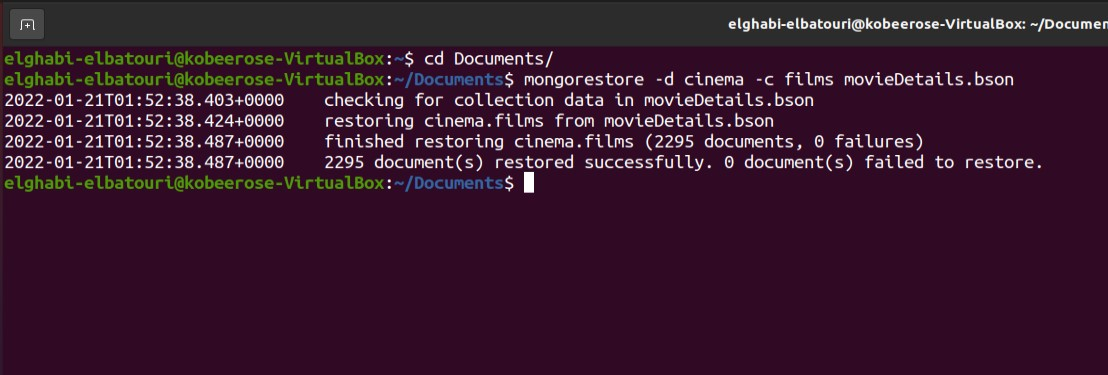
\includegraphics[width=.93\linewidth]{Pictures/MongoDB/Examining MongoDB Query Features/Restoring a .bson file/Restore movieDetails in the DB} 
\end{center} 
\caption{Restore movieDetails in the DB} 
\end{figure}  \FloatBarrier
\\
\par Okay, so let's test some command on our Database.
\begin{figure}[!htb] 
\begin{center} 
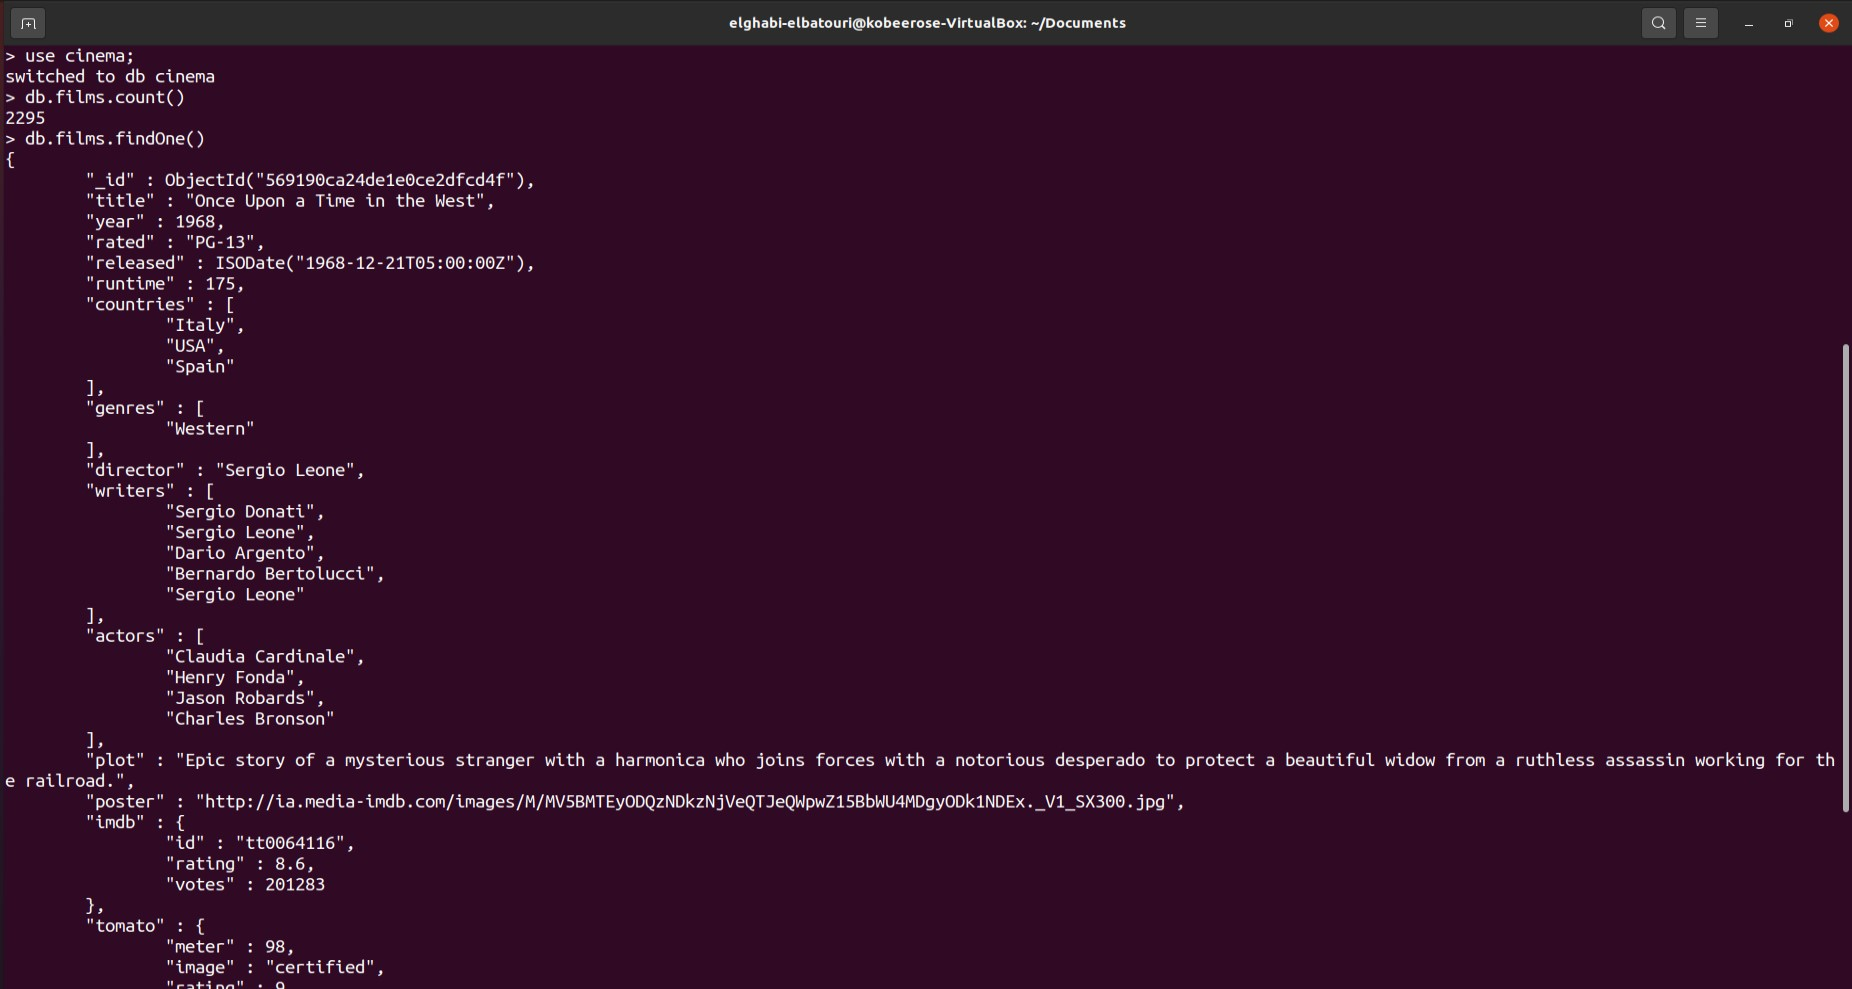
\includegraphics[width=.93\linewidth]{Pictures/MongoDB/Examining MongoDB Query Features/Restoring a .bson file/Checking the data in mongo shell} 
\end{center} 
\caption{Checking the data in mongo shell} 
\end{figure}  \FloatBarrier
\\
\section{Index management }
\par Display of all indexes in the Database.
\\
\begin{figure}[!htb] 
\begin{center} 
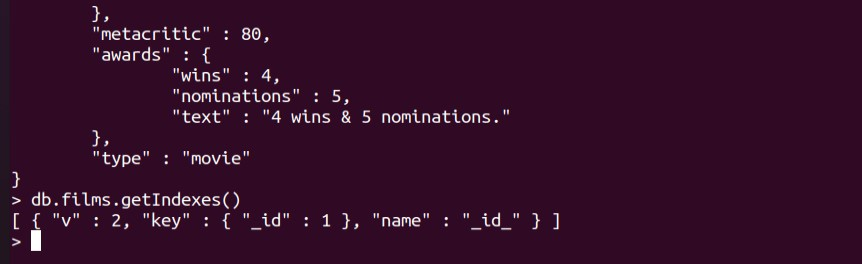
\includegraphics[width=1\linewidth]{Pictures/MongoDB/Examining MongoDB Query Features/Index management/Displaying indexes} 
\end{center} 
\caption{Displaying indexes} 
\end{figure}  \FloatBarrier
\\

\par Here is an example of creating a new "genre" index whose field must be
necessarily present.
\\
\begin{figure}[!htb] 
\begin{center} 
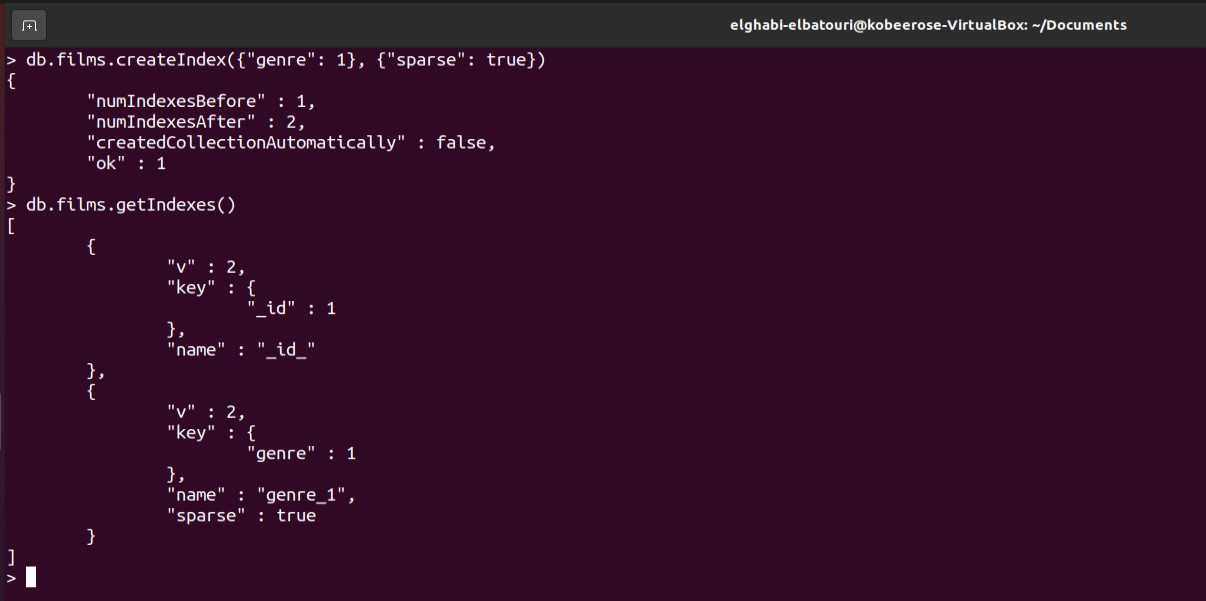
\includegraphics[width=1\linewidth]{Pictures/MongoDB/Examining MongoDB Query Features/Index management/Creating an Index} 
\end{center} 
\caption{Creating an Index} 
\end{figure}  \FloatBarrier
\\
\newpage
\par We can delete an index with the command dropIndex.
\\
\begin{figure}[!htb] 
\begin{center} 
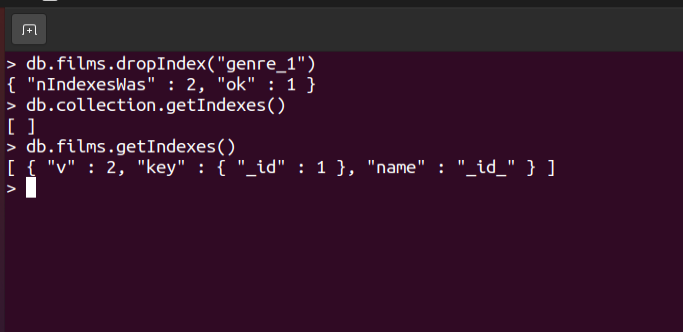
\includegraphics[width=1\linewidth]{Pictures/MongoDB/Examining MongoDB Query Features/Index management/Dropping an index} 
\end{center} 
\caption{Dropping an index} 
\end{figure}  \FloatBarrier
\\

\par When searching for a given document, it is possible to know the effective strategy
allowing MongoDB to find it using the explain() command.
\\
\begin{figure}[!htb] 
\begin{center} 
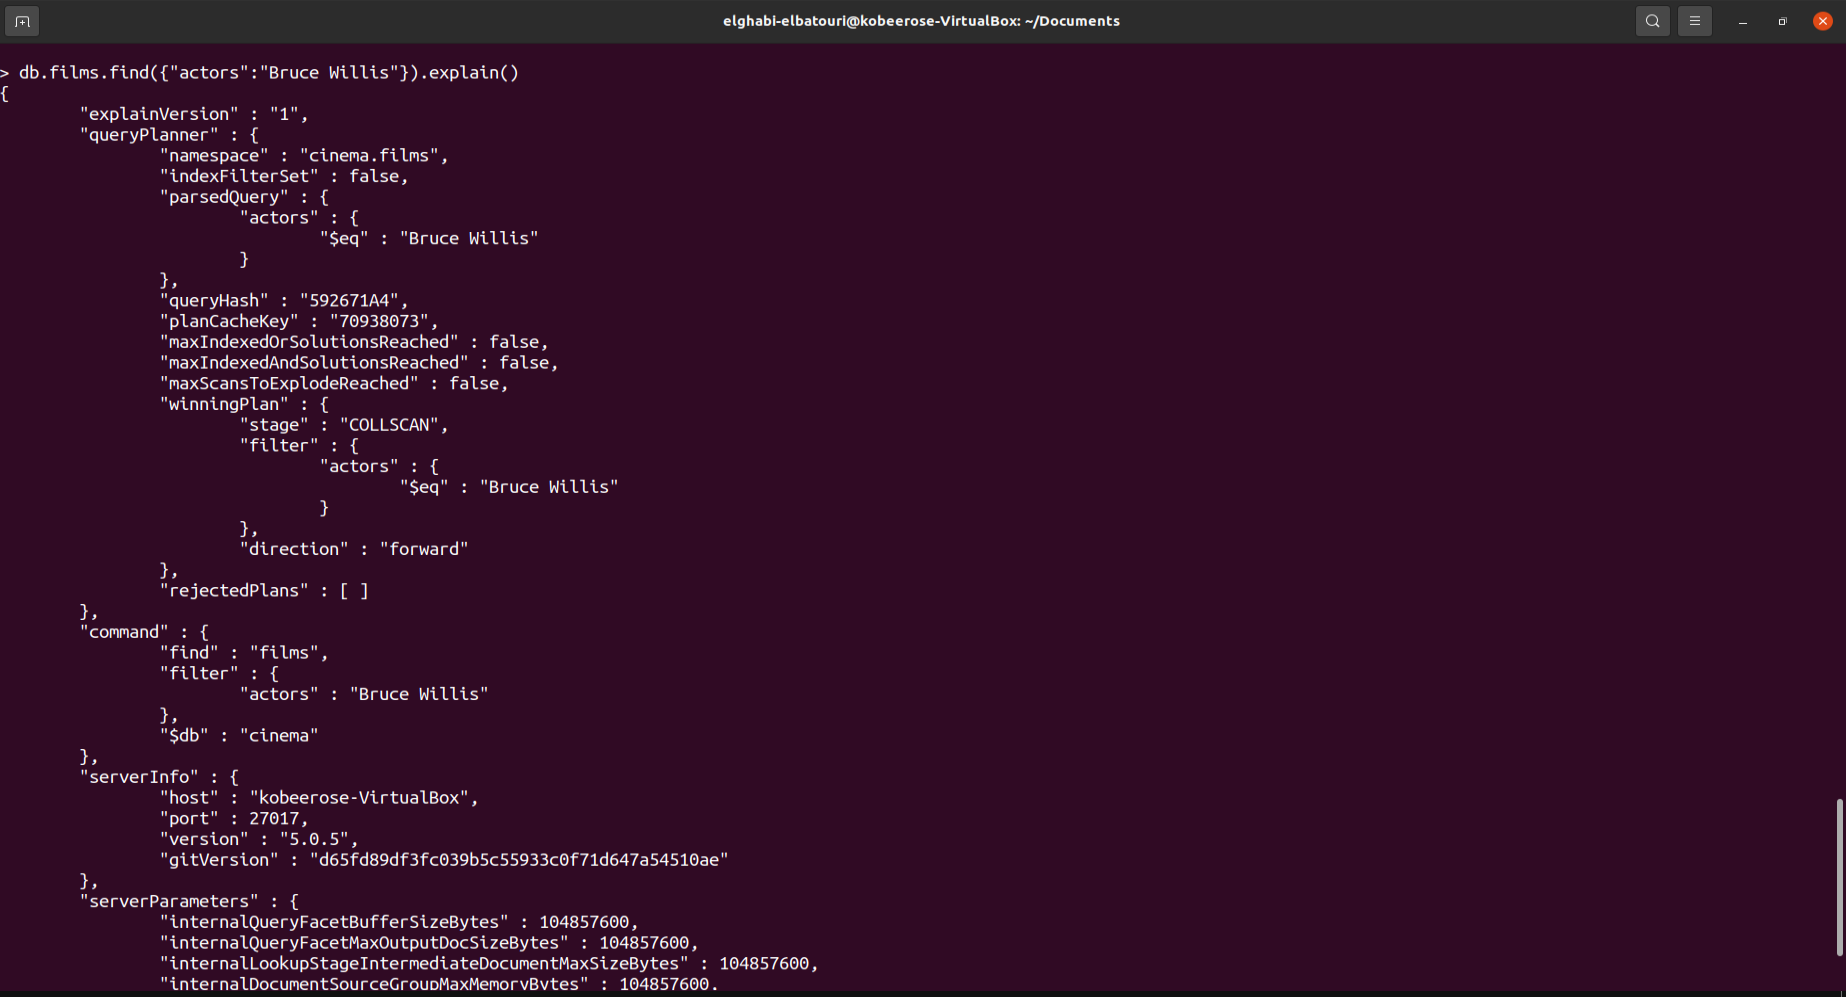
\includegraphics[width=1\linewidth]{Pictures/MongoDB/Examining MongoDB Query Features/Index management/explain() command} 
\end{center} 
\caption{explain() command} 
\end{figure}  \FloatBarrier
\\
\newpage
\section{Document search }
\par To search for a document, we need to place a condition in the find command.
This condition is described in a JSON document.
\\
\begin{figure}[!htb] 
\begin{center} 
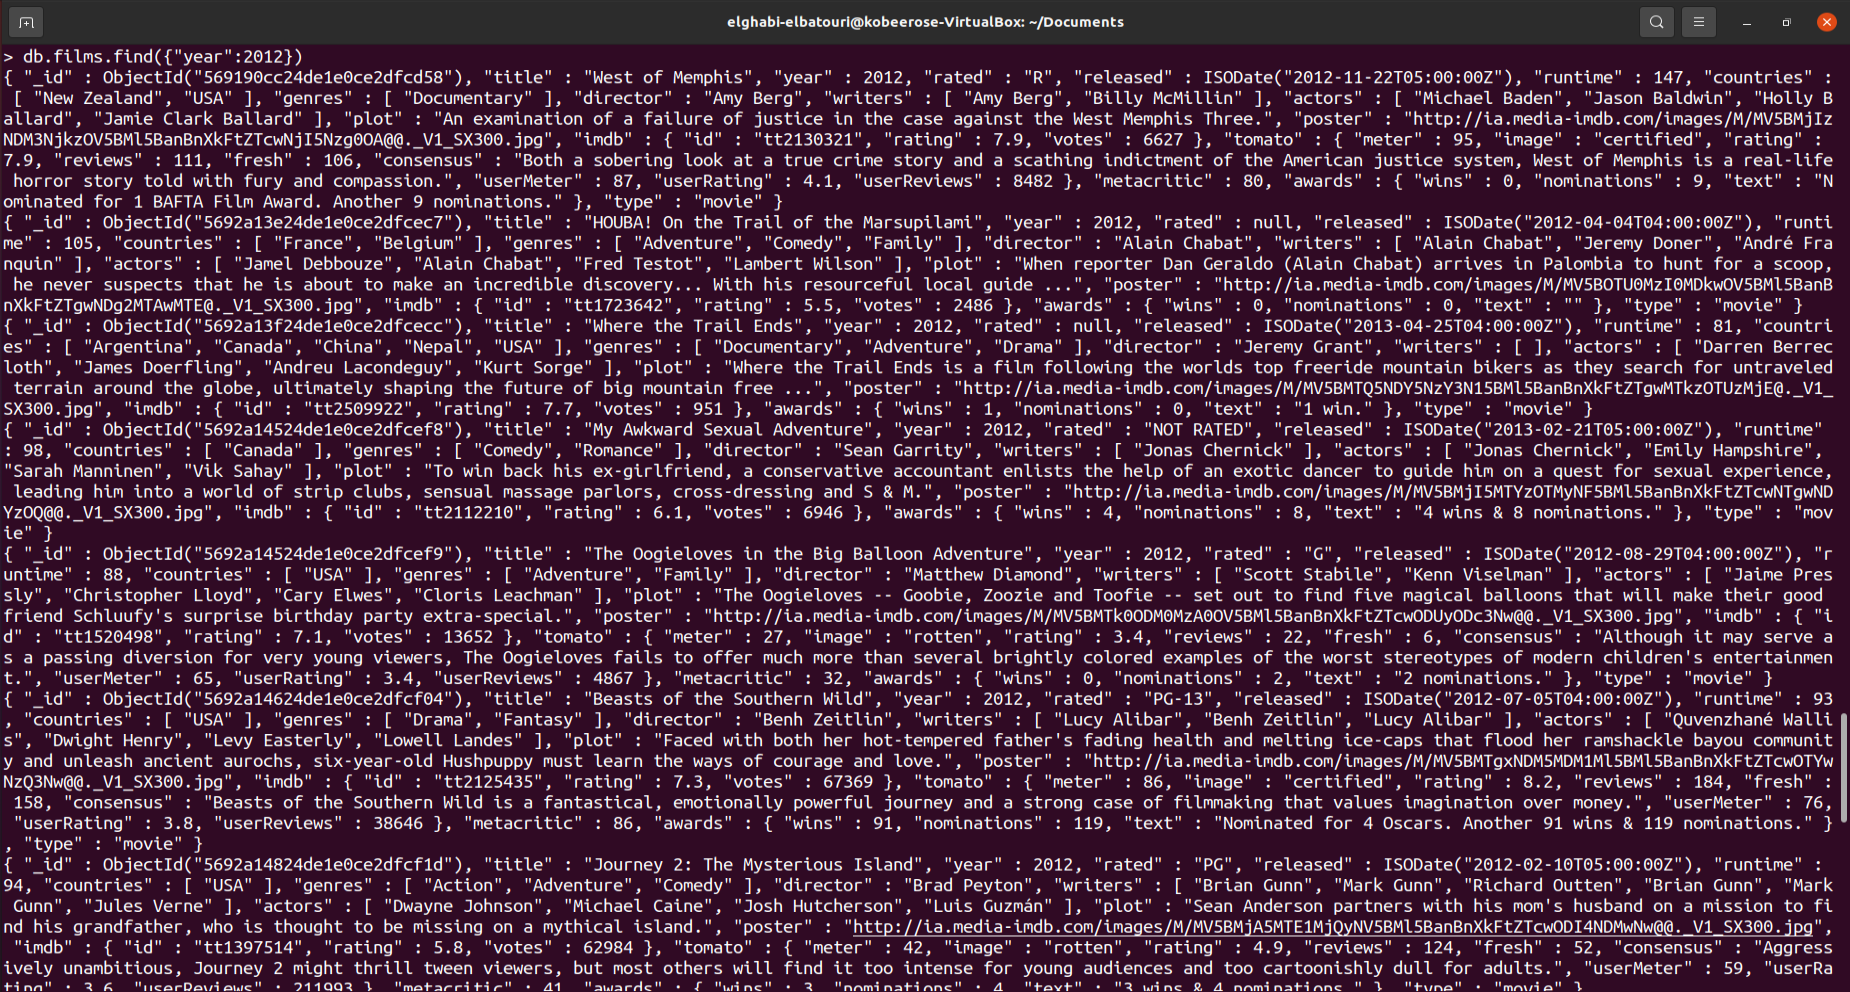
\includegraphics[width=1\linewidth]{Pictures/MongoDB/Examining MongoDB Query Features/Document search/Searching for 2012 films} 
\end{center} 
\caption{Searching for 2012 films} 
\end{figure}  \FloatBarrier
\\

\par To improve the display, We can use the pretty command.
\\
\begin{figure}[!htb] 
\begin{center} 
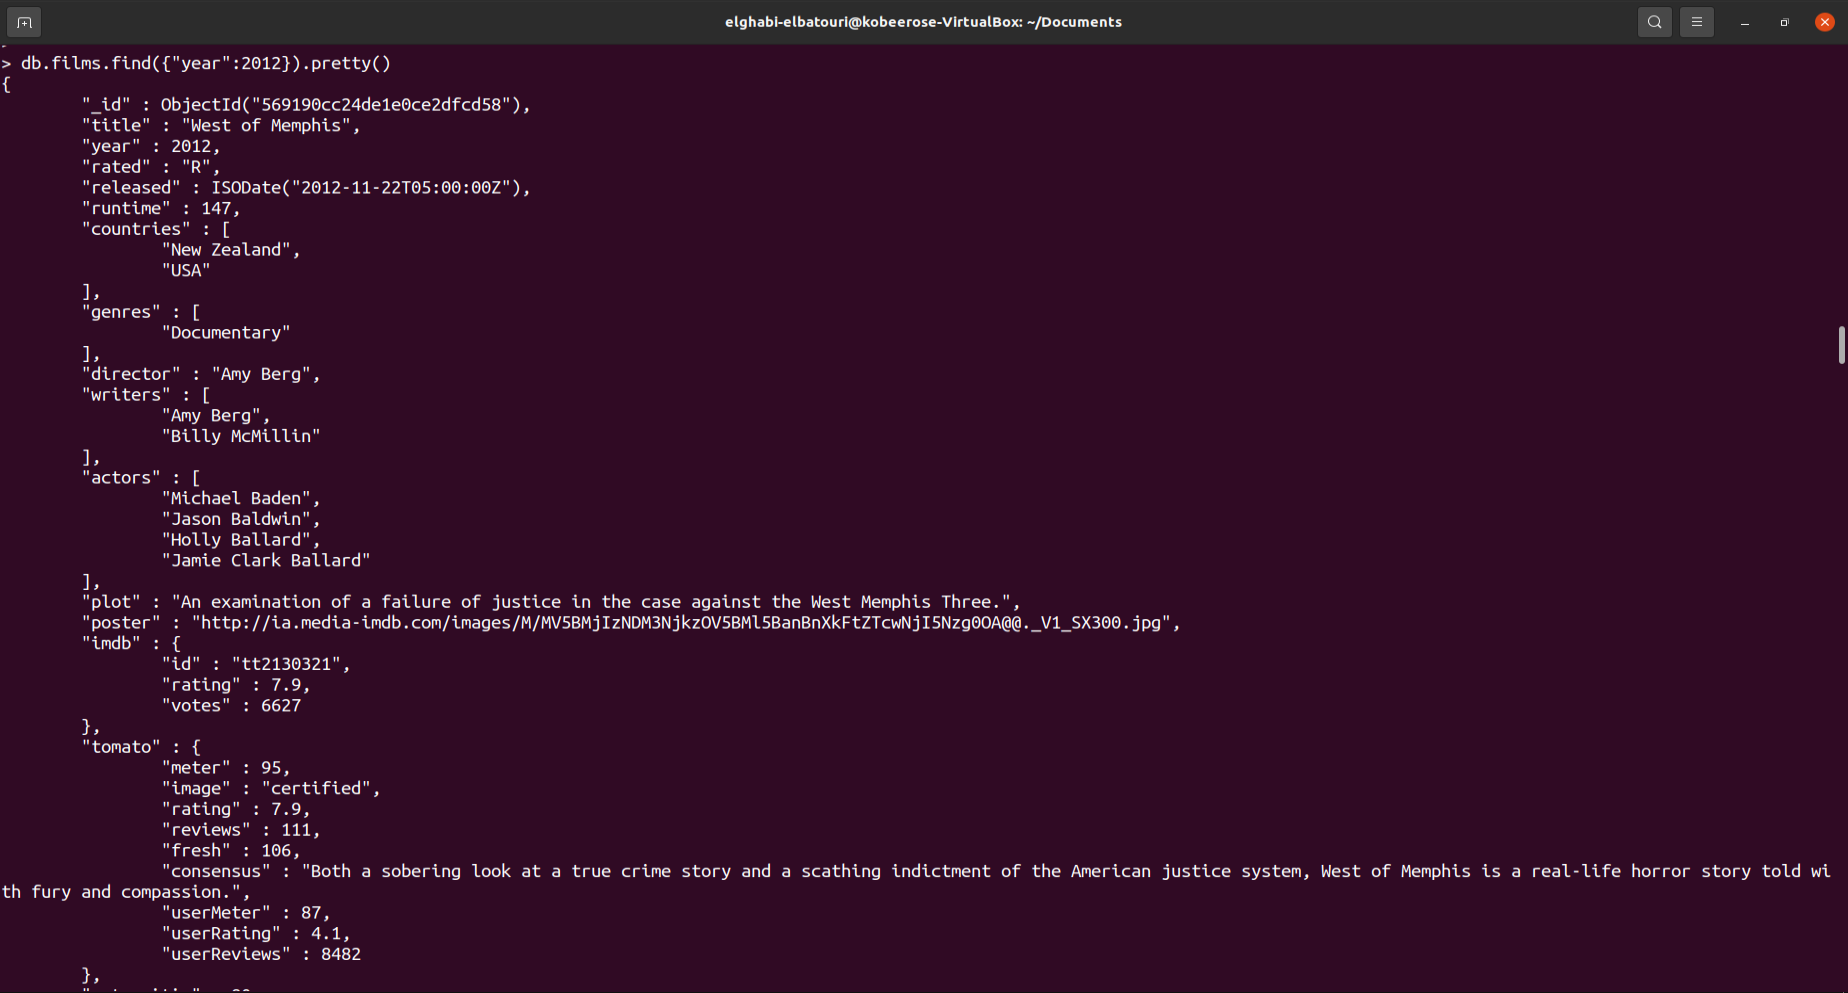
\includegraphics[width=1\linewidth]{Pictures/MongoDB/Examining MongoDB Query Features/Document search/Formatting the search results} 
\end{center} 
\caption{Formatting the search results} 
\end{figure}  \FloatBarrier
\\
\newpage
\par The projection makes it possible to select the information to be returned. We will limit the information returned by specifying the desired fields in a JSON document. And, also pass this document as the second argument of my find search.
\\
\begin{figure}[!htb] 
\begin{center} 
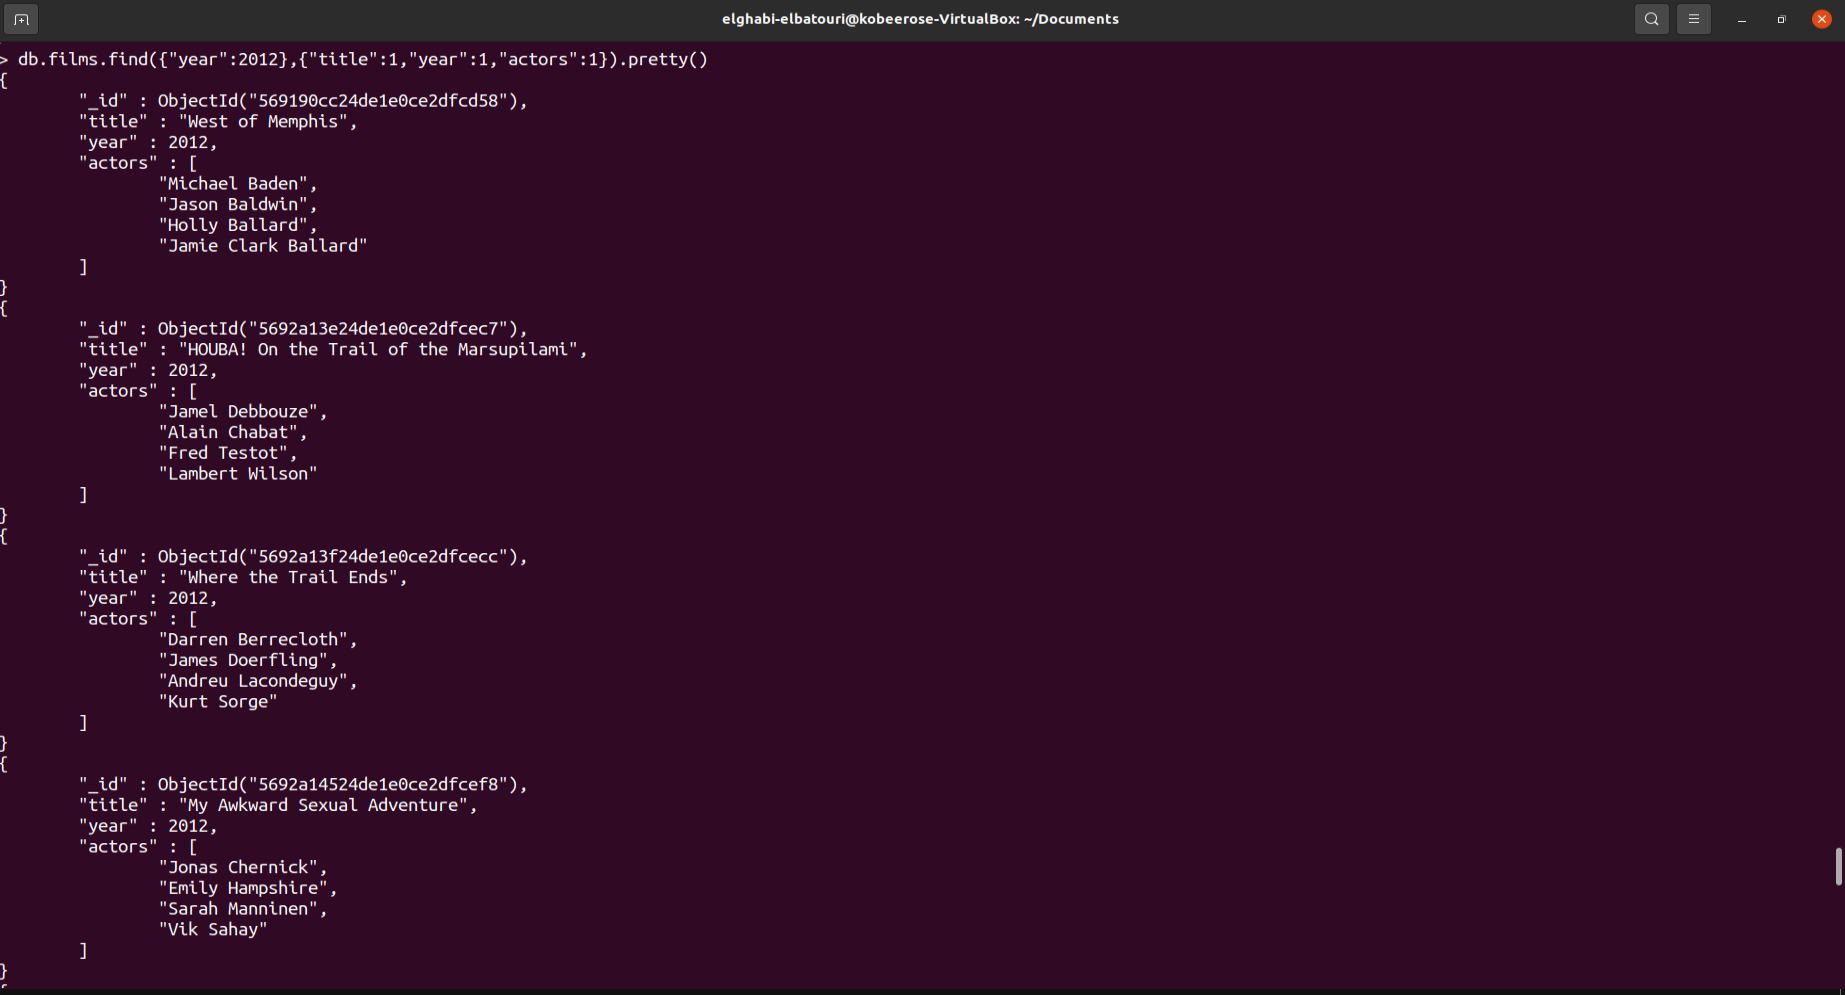
\includegraphics[width=1\linewidth]{Pictures/MongoDB/Examining MongoDB Query Features/Document search/Projection} 
\end{center} 
\caption{Projection} 
\end{figure}  \FloatBarrier
\\

\par To keep a field, we will simply specify it in this document and assign it the value 1.
We will also have noticed that the query also returned the \_id field. 
\\
\begin{figure}[!htb] 
\begin{center} 
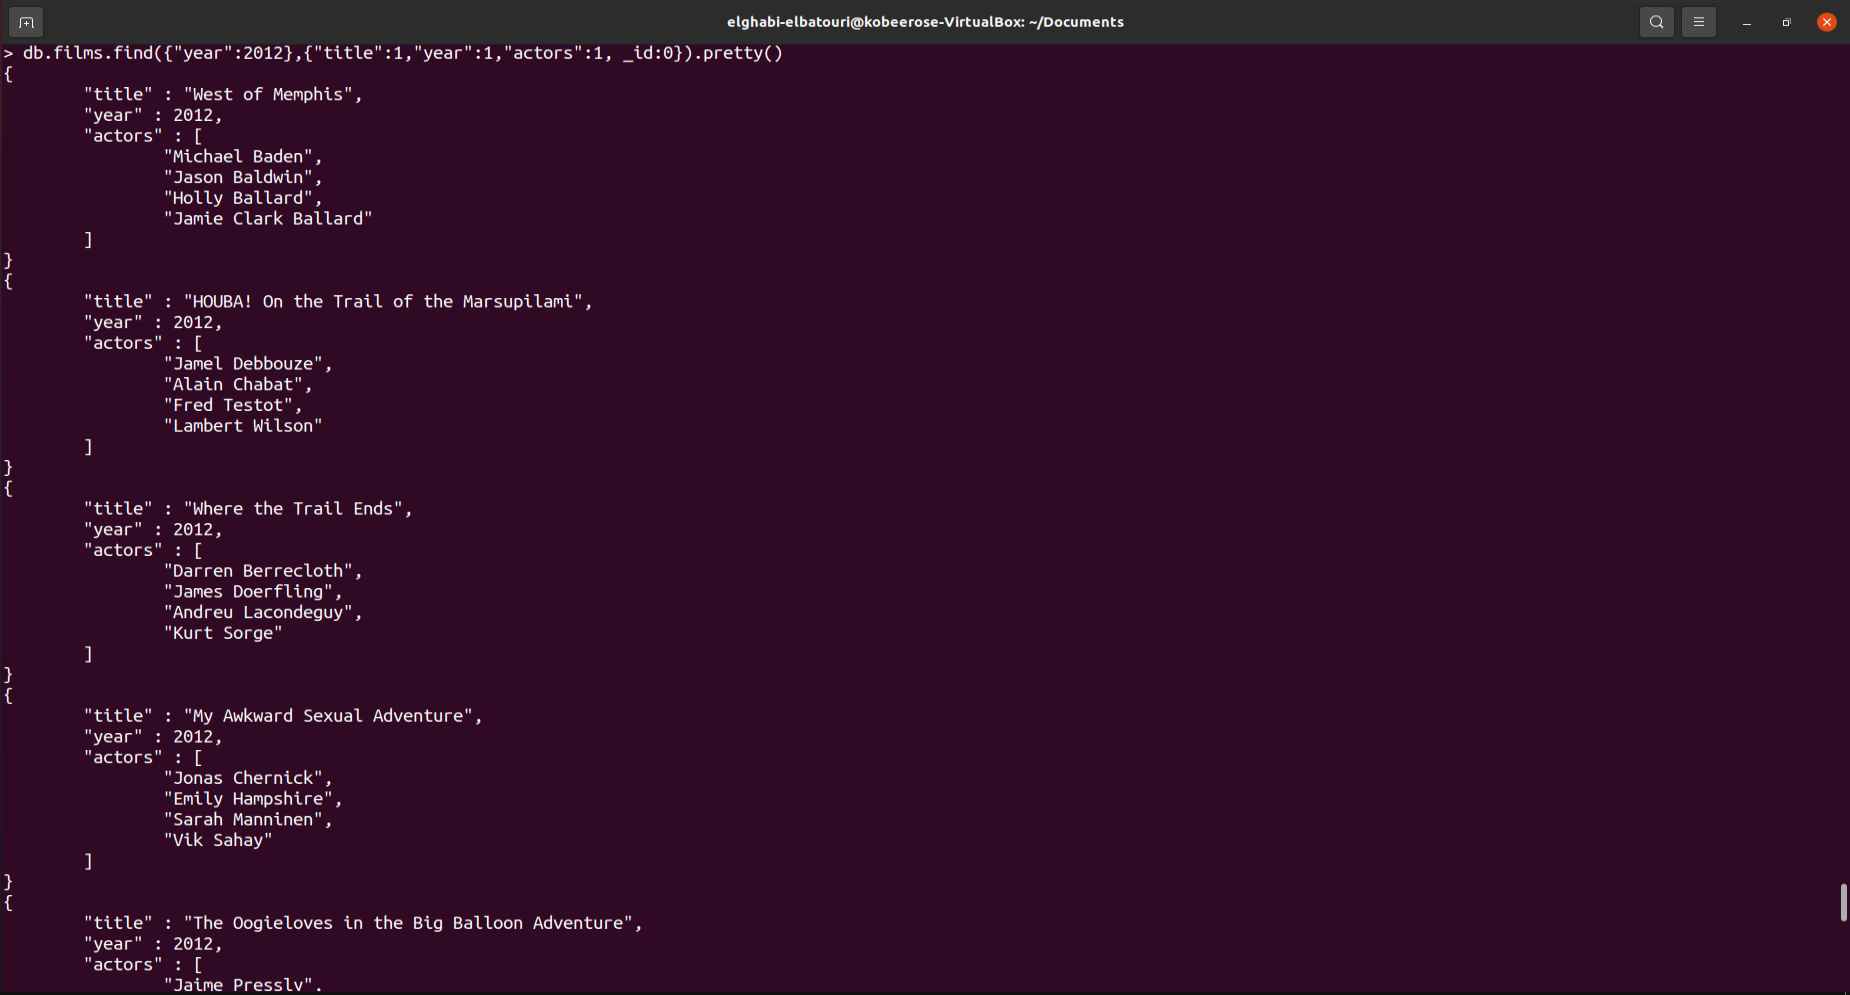
\includegraphics[width=1\linewidth]{Pictures/MongoDB/Examining MongoDB Query Features/Document search/Including and excluding fields} 
\end{center} 
\caption{Including and excluding fields} 
\end{figure}  \FloatBarrier
\\
\newpage
\par Let's get The documents containing simple fields such as the year or the title of the film but also
arrays to store actor names.
\\
\begin{figure}[!htb] 
\begin{center} 
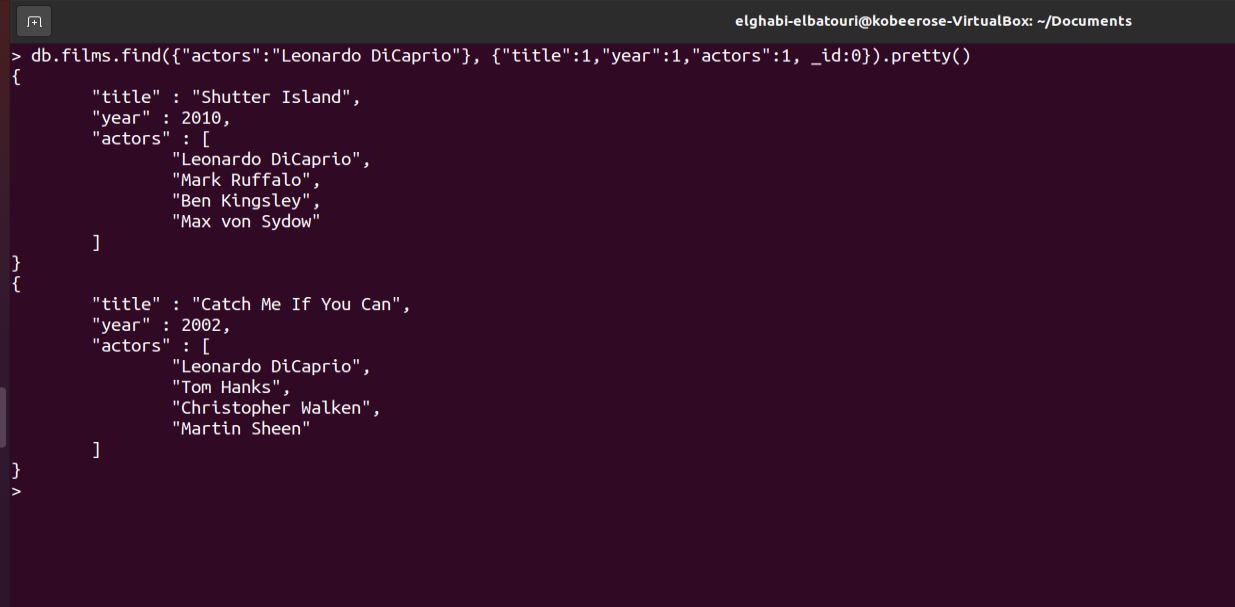
\includegraphics[width=1\linewidth]{Pictures/MongoDB/Examining MongoDB Query Features/Document search/Searching in tables} 
\end{center} 
\caption{Searching in tables} 
\end{figure}  \FloatBarrier
\\

\par We can combine multiple filters.
\\
\begin{figure}[!htb] 
\begin{center} 
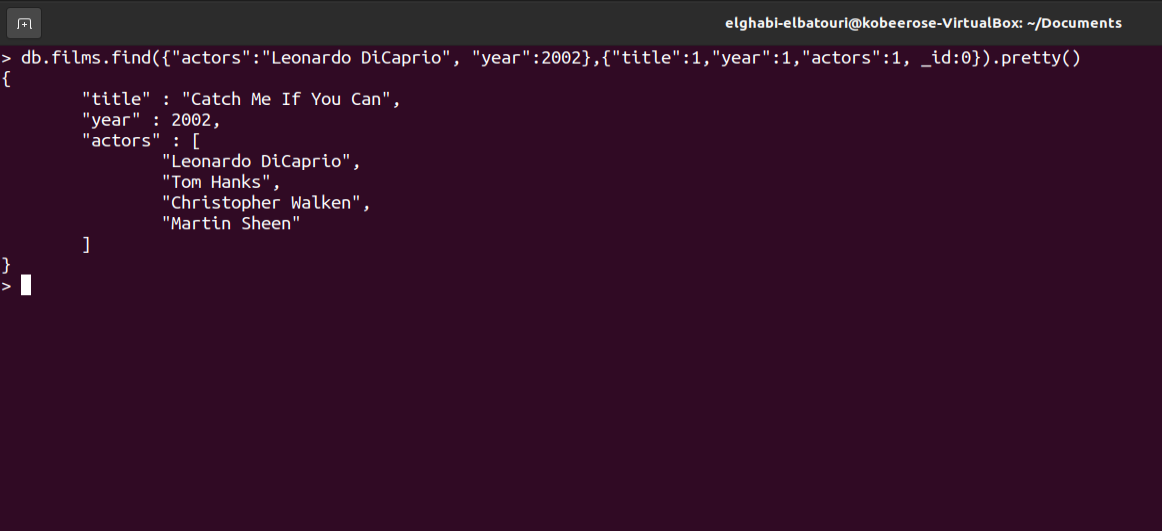
\includegraphics[width=1\linewidth]{Pictures/MongoDB/Examining MongoDB Query Features/Document search/Combining multiple filters} 
\end{center} 
\caption{Combining multiple filters} 
\end{figure}  \FloatBarrier
\\
\newpage
\par We want to filter out movies with Leonardo DiCaprio or Tom Hanks. For this we will use
the \$in operator.
\\
\begin{figure}[!htb] 
\begin{center} 
\includegraphics[width=1\linewidth]{Pictures/MongoDB/Examining MongoDB Query Features/Document search/Using \$in operator} 
\end{center} 
\caption{Using \$in operator} 
\end{figure}  \FloatBarrier
\\

\par To have only the films with Leonardo DiCaprio and Tom Hanks, there is the operator \$all
\\
\begin{figure}[!htb] 
\begin{center} 
\includegraphics[width=1\linewidth]{Pictures/MongoDB/Examining MongoDB Query Features/Document search/Using \$all operator} 
\end{center} 
\caption{Using \$all operator} 
\end{figure}  \FloatBarrier
\\
\newpage
\section{Advanced search }
\par MongoDB's query language is extremely powerful. It allows us to perform all
possible requests and the objective of this lab is not to make an exhaustive list of them. We'll just
end with some slightly more advanced research.
\\
\begin{figure}[!htb] 
\begin{center} 
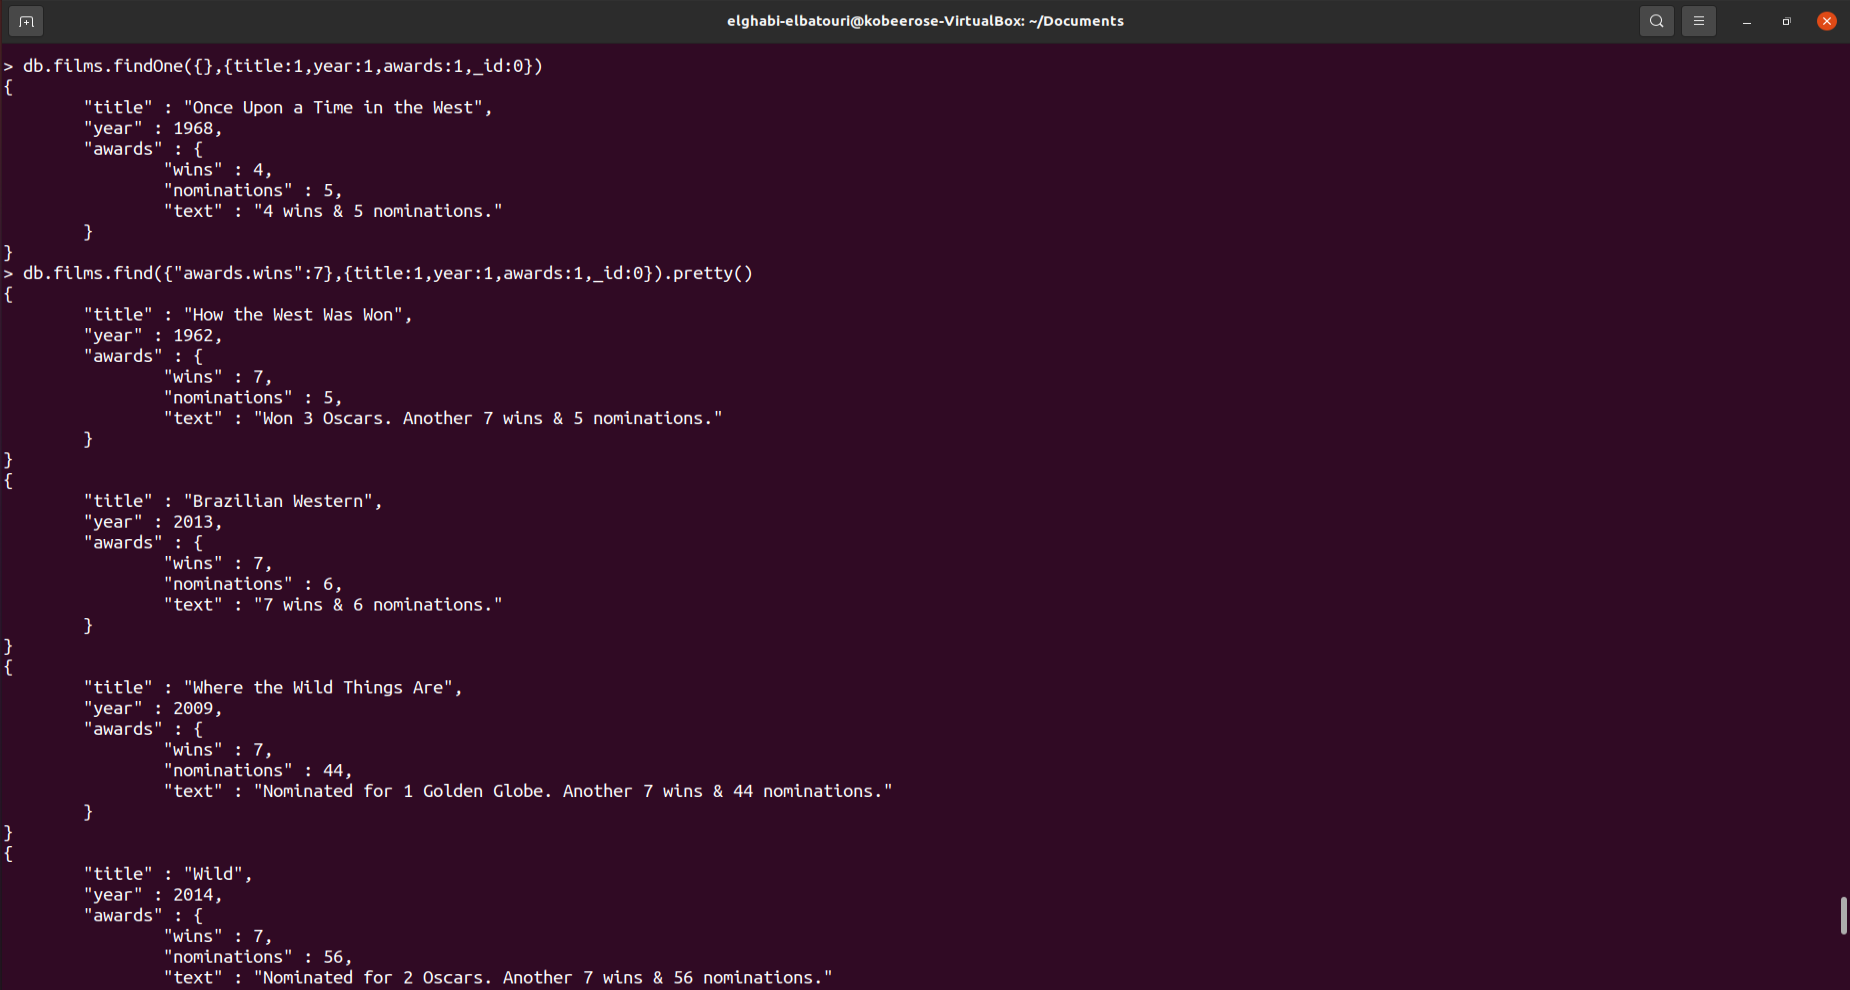
\includegraphics[width=1\linewidth]{Pictures/MongoDB/Examining MongoDB Query Features/Advanced search/Checking nested documents} 
\end{center} 
\caption{Checking nested documents} 
\end{figure}  \FloatBarrier
\\

\par A search for all films that have won at least one award using the \$ne.
\\
\begin{figure}[!htb] 
\begin{center} 
\includegraphics[width=1\linewidth]{Pictures/MongoDB/Examining MongoDB Query Features/Advanced search/Using \$ne operator} 
\end{center} 
\caption{Using \$ne operator} 
\end{figure}  \FloatBarrier
\\
\newpage
\par We search for films that have won more than 80 awards using the \$gte.
\\
\begin{figure}[!htb] 
\begin{center} 
\includegraphics[width=1\linewidth]{Pictures/MongoDB/Examining MongoDB Query Features/Advanced search/Using \$gte operator} 
\end{center} 
\caption{Using \$gte operator} 
\end{figure}  \FloatBarrier
\\

\par We will next resume our previous query and sort the results by descending order on the number of prizes obtained.
\\
\begin{figure}[!htb] 
\begin{center} 
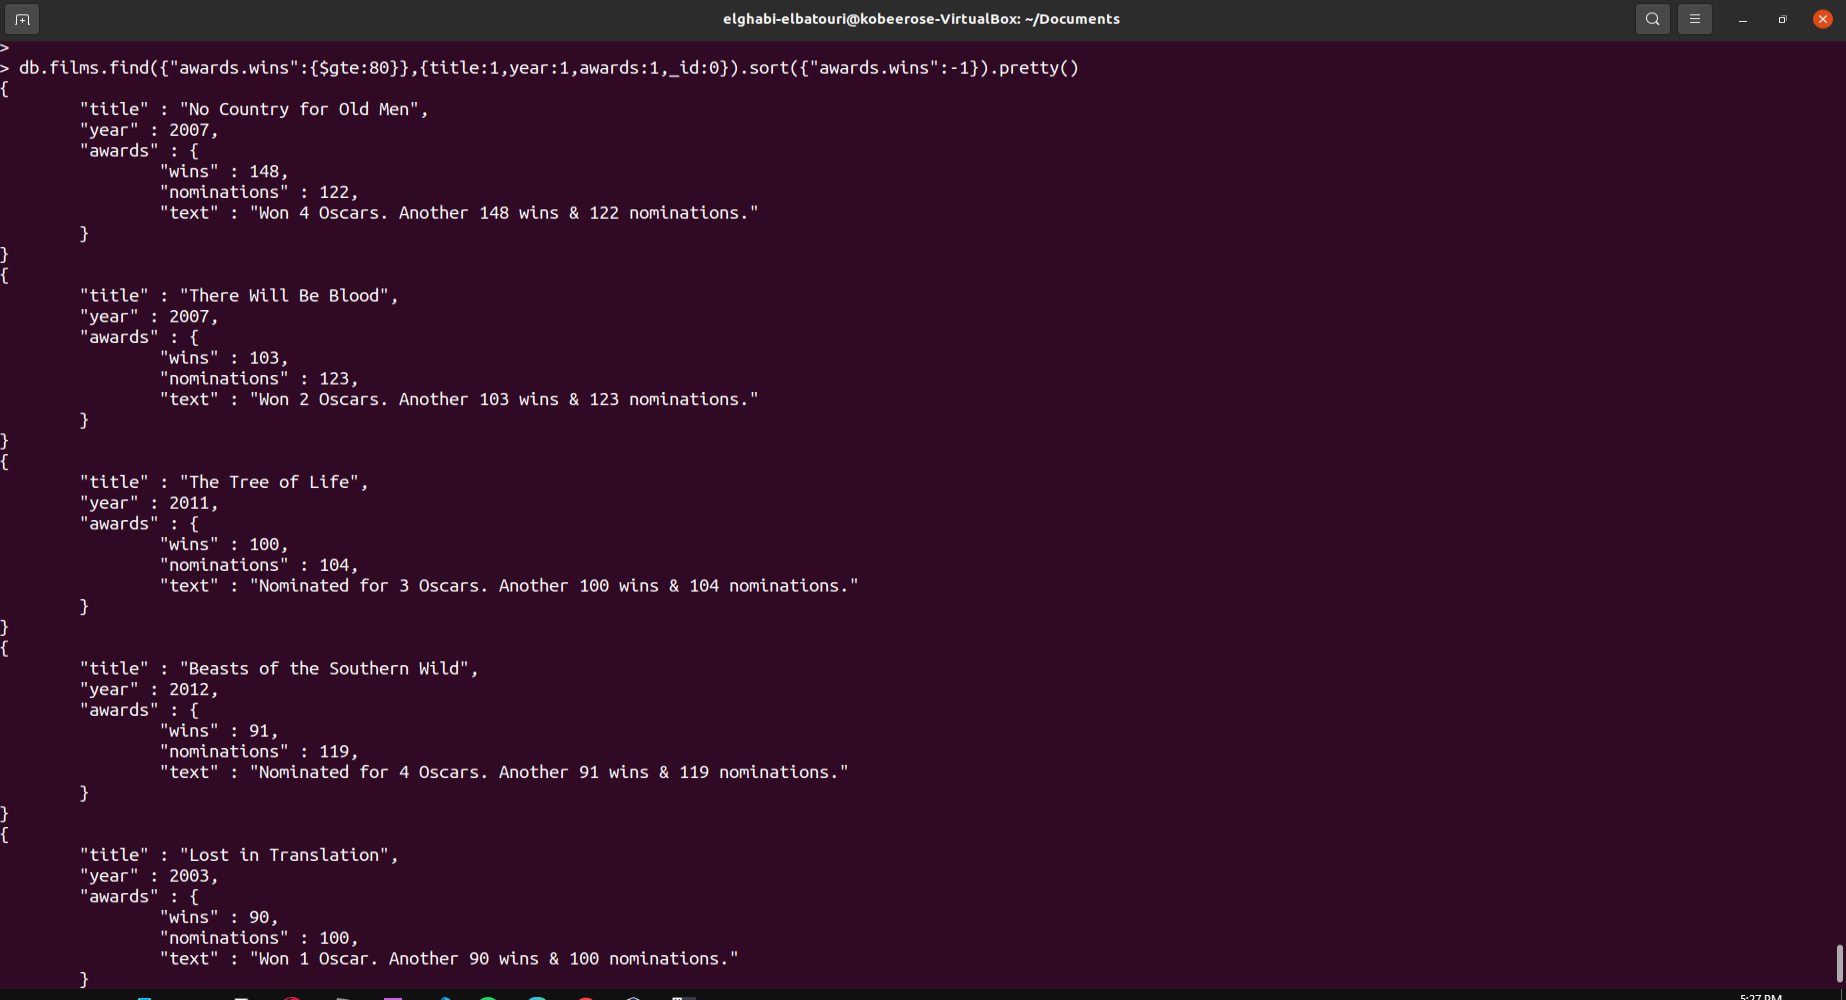
\includegraphics[width=1\linewidth]{Pictures/MongoDB/Examining MongoDB Query Features/Advanced search/Sorting results} 
\end{center} 
\caption{Sorting results} 
\end{figure}  \FloatBarrier
\\
\section{Inserting documents }
\par We will start by inserting a document using the insertOne() function. Then we verify the db using the find() function. When we look at the collection, we can see that MongoDB has inserted the document. He created also a key, named \_id
\\
\begin{figure}[!htb] 
\begin{center} 
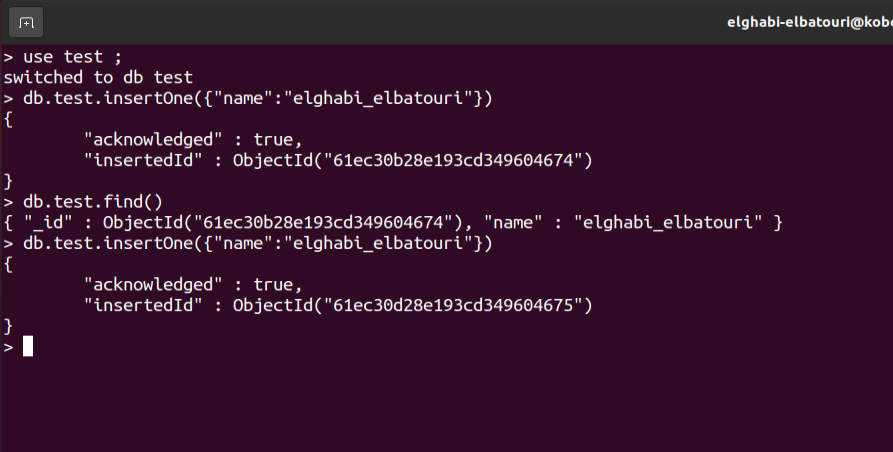
\includegraphics[width=1\linewidth]{Pictures/MongoDB/Examining MongoDB Query Features/Inserting documents/Inserting object and checking} 
\end{center} 
\caption{Inserting object and checking} 
\end{figure}  \FloatBarrier
\\

\par Now we redo the same insertion, as we can see MongoDB inserted a second document. The system did not detect a duplicate: it generated a different key for the two records.
We can decide to take control and define the \_id key ourselves. So, if we try this time to insert a name with the same \_id:0, it will generate an error.
\\
\begin{figure}[!htb] 
\begin{center} 
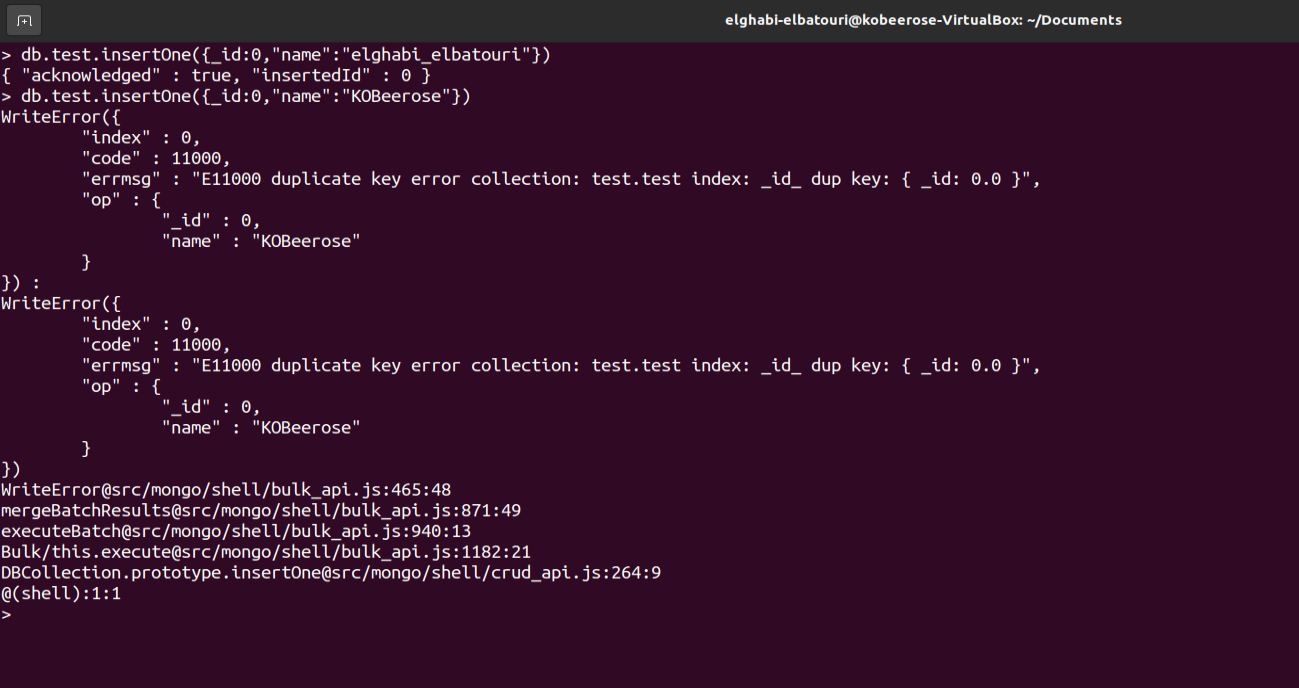
\includegraphics[width=1\linewidth]{Pictures/MongoDB/Examining MongoDB Query Features/Inserting documents/Error of inserting in the same id} 
\end{center} 
\caption{Error of inserting in the same id} 
\end{figure}  \FloatBarrier
\\
\newpage
\par We can as well insert a document with a different structure in the same collection. It is possible likewise to insert several documents at the same time. We will pass an array as an argument
of documents to the insert() function.
\\
\begin{figure}[!htb] 
\begin{center} 
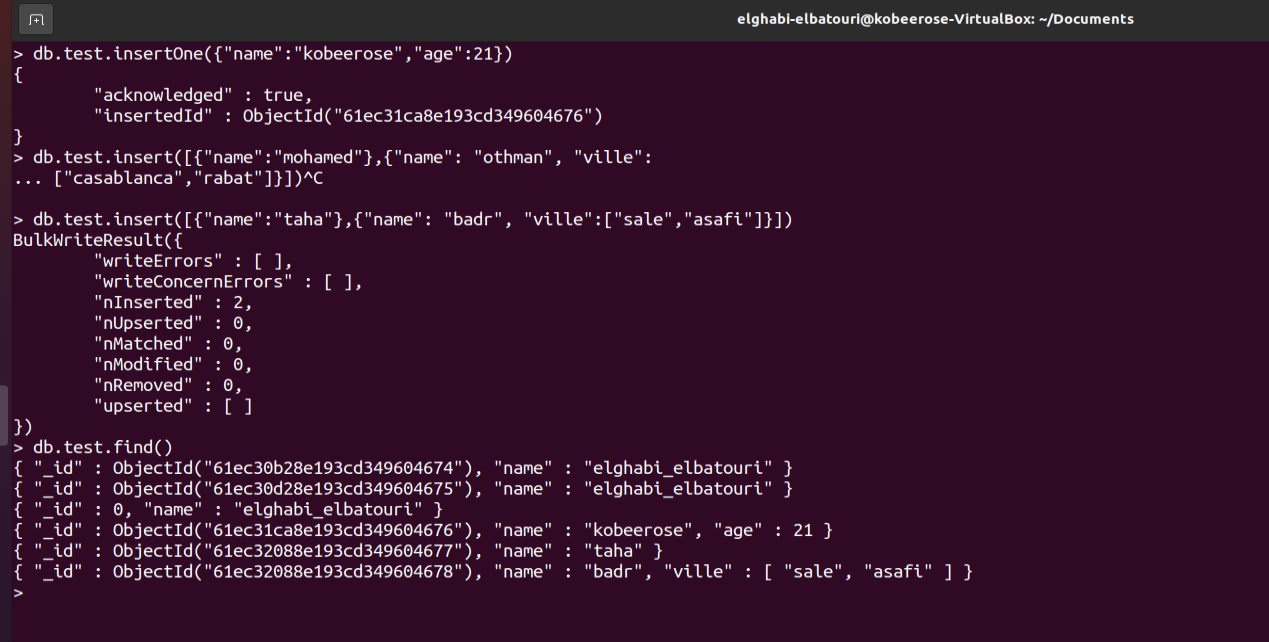
\includegraphics[width=1\linewidth]{Pictures/MongoDB/Examining MongoDB Query Features/Inserting documents/Documents with different structure in same collection} 
\end{center} 
\caption{Documents with different structure in same collection} 
\end{figure}  \FloatBarrier
\\
\section{Deleting and Updating documents }
\par To delete a collection, we use the drop() function. We can then verify that the collection
no longer contains any documents.
\\
\begin{figure}[!htb] 
\begin{center} 
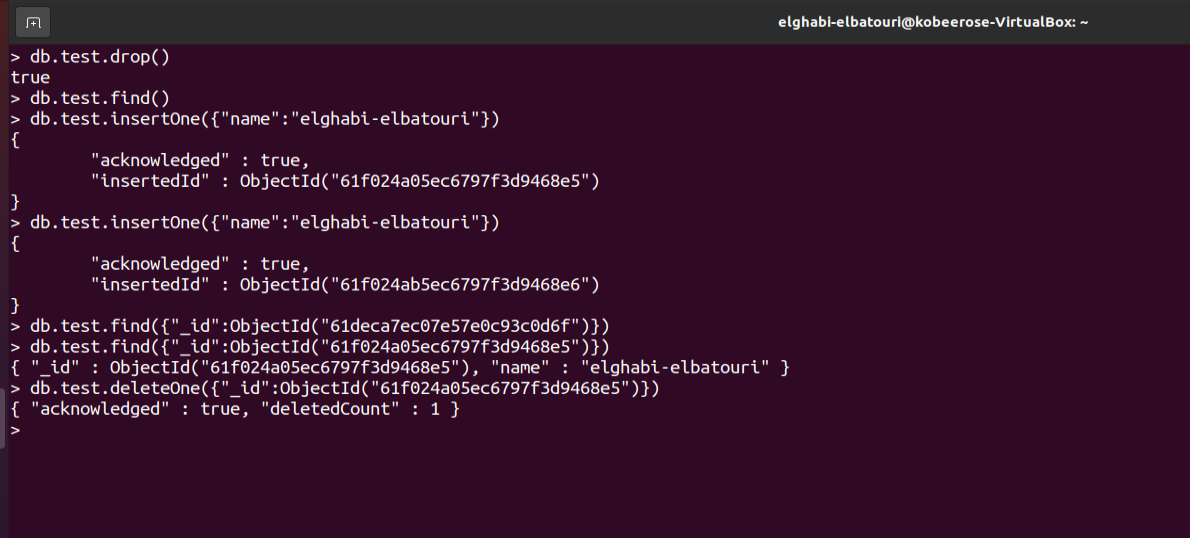
\includegraphics[width=1\linewidth]{Pictures/MongoDB/Examining MongoDB Query Features/Deleting and Updating documents/Delete documents} 
\end{center} 
\caption{Delete documents} 
\end{figure}  \FloatBarrier
\\
\newpage
\par MongoDB provides the update function with different operators depending on the update type.
desired day. The update function takes two required arguments:\\
\begin{itemize}
  \item a document representing the search condition for the documents in the collection,
  \item a document representing the desired update.
  \item
\end{itemize}

So we can add or replace an existing field with \$set
\\
\begin{figure}[!htb] 
\begin{center} 
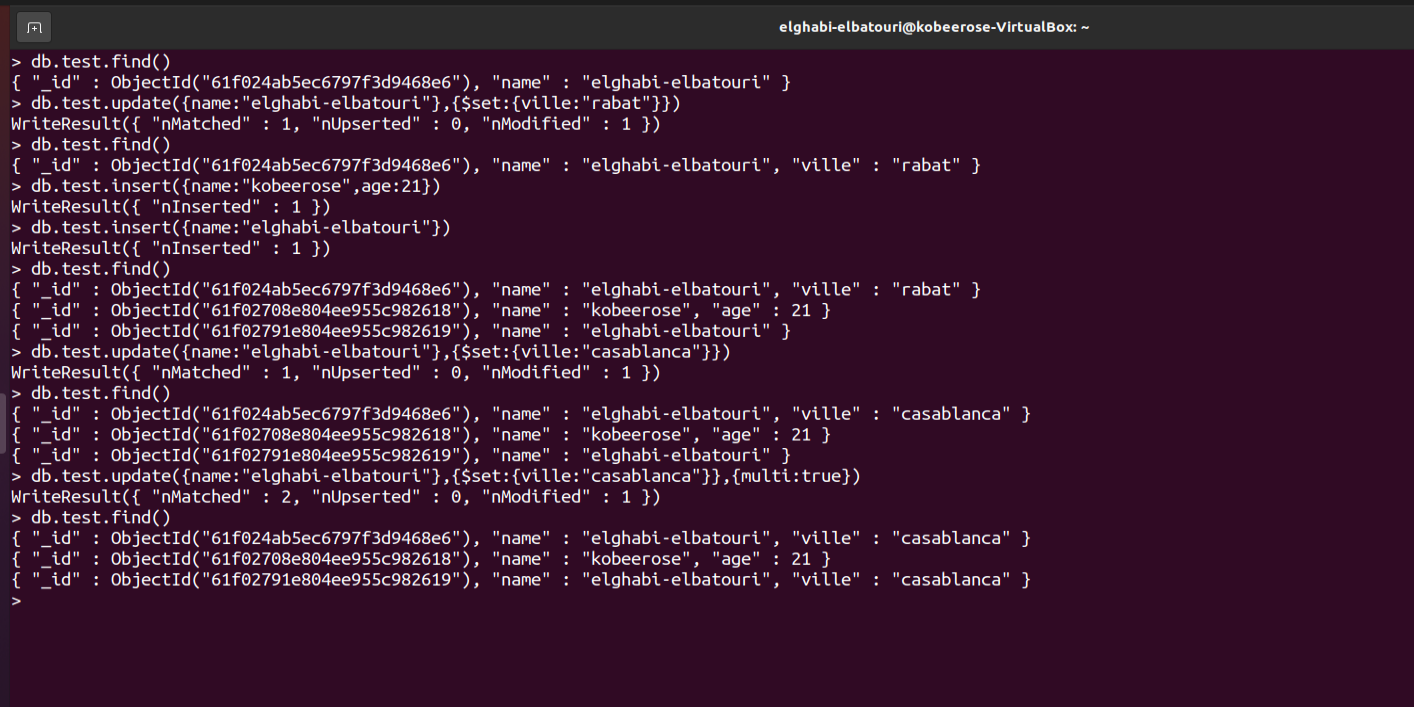
\includegraphics[width=1\linewidth]{Pictures/MongoDB/Examining MongoDB Query Features/Deleting and Updating documents/Updating documents} 
\end{center} 
\caption{Updating documents} 
\end{figure}  \FloatBarrier
\\

\par Now let's Increment an existing numeric field with the \$inc operator.
\\
\begin{figure}[!htb] 
\begin{center} 
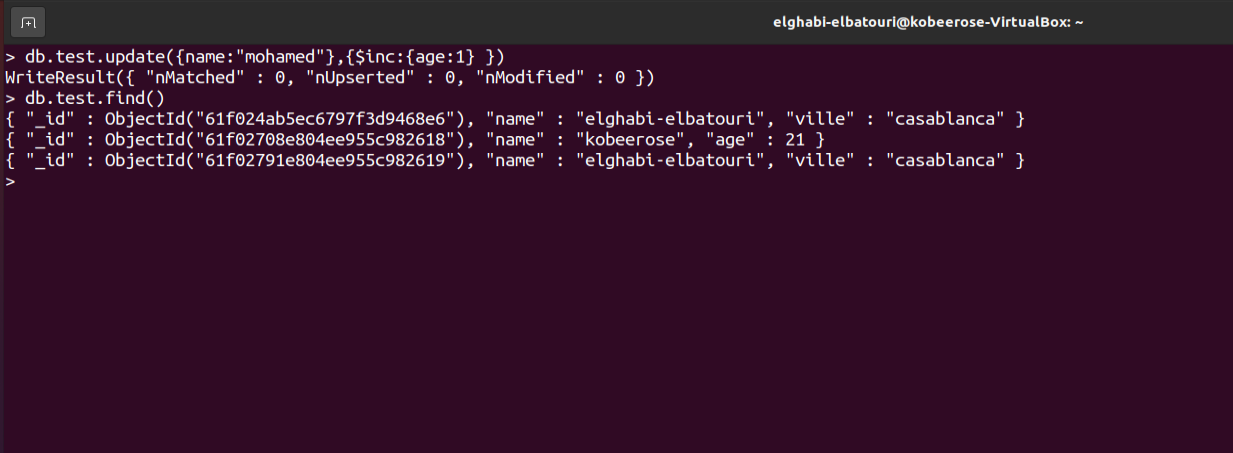
\includegraphics[width=1\linewidth]{Pictures/MongoDB/Examining MongoDB Query Features/Deleting and Updating documents/Increment a numeric field} 
\end{center} 
\caption{Increment a numeric field} 
\end{figure}  \FloatBarrier
\\
\newpage
\par We can update table without overwriting existing data
using \$push operator adds a new element to an array and remove an element we can use \$pull.
\\
\begin{figure}[!htb] 
\begin{center} 
\includegraphics[width=1\linewidth]{Pictures/MongoDB/Examining MongoDB Query Features/Deleting and Updating documents/Using \$push or \$pull operators} 
\end{center} 
\caption{Using \$push or \$pull operators} 
\end{figure}  \FloatBarrier

\end{spacing}